\documentclass[center]{beamer}

\usetheme[compress]{Singapore}

% Do not show subsection markers in the headline 
\setbeamertemplate{Singapore subsection in head/foot}{use=false}
% Remove navigation symbols in the bottom of the slides
\beamertemplatenavigationsymbolsempty 
% \newcommand\independent{\protect\mathpalette{\protect\independenT}{\perp}}
% \def\independenT#1#2{\mathrel{\rlap{$#1#2$}\mkern2mu{#1#2}}}


\usepackage{marvosym}
\usepackage{graphicx}
\usepackage[backend      = biber,     
            isbn         = false,     
            doi          = false,     
            url          = false,     
            eprint       = false,    
            style        = alphabetic,
            maxcitenames = 1,         
            maxbibnames  = 3,         
            uniquelist   = false]{biblatex}
\addbibresource{/home/bach/Documents/papers/BIB/references.bib}
\usepackage{amsmath}
\usepackage{amsthm}
\usepackage{amsfonts}
\usepackage{amssymb}
\usepackage{mathtools}
\mathtoolsset{showonlyrefs=true}
\usepackage{booktabs}

\theoremstyle{definition}
\newtheorem{mydef}{Definition}[section]

\newcommand{\ex}[1]{{\usebeamercolor[fg]{block title example} #1}}


% Configure title, authors and contact 
\title[Retention order prediction]{%
    Liquid-Chromatography Retention Order Prediction for Metabolite Identification}
    
\author[\Letter: eric.bach@aalto.fi]{ % address for correspondence 
    Eric Bach\,$^{\text{1,\Letter}}$, % 
    Sandor Szedmak\,$^{\text{1}}$,    %
    C\'eline Brouard\,$^{\text{1}}$,  %
    Sebastian B\"ocker\,$^{\text{2}}$ %
    and Juho Rousu\,$^{\text{1}}$}
    
\institute[]{%
    $^{\text{1}}$Helsinki institute for Information Technology (HIIT), Department of Computer Science, Aalto University, Espoo, Finland\\
    $^{\text{2}}$Chair for Bioinformatics, Friedrich-Schiller-University, Jena, Germany.}
  \date{September 11, 2018}

% Configure beamer footline
\setbeamertemplate{footline}{%
    \leavevmode%
    \hbox{%
        \hskip3pt
        \begin{beamercolorbox}[wd=.69\paperwidth,ht=2.25ex,dp=1ex,left]{title in head/foot}%
            \usebeamerfont{title in head/foot}\inserttitle
        \end{beamercolorbox}
        \begin{beamercolorbox}[wd=.15\paperwidth,ht=2.25ex,dp=1ex,center]{author in head/foot}%
            \usebeamerfont{author in head/foot}\insertshortauthor
        \end{beamercolorbox}
        \begin{beamercolorbox}[wd=.15\paperwidth,ht=2.25ex,dp=1ex,right]{framenumber in head/foot}%
            \insertframenumber{} / \inserttotalframenumber\hspace{7pt}
        \end{beamercolorbox}
  }%
  \vskip0pt%
}

% \setbeamertemplate{headline}
% {
%     \leavevmode
%     \begin{beamercolorbox}{section in head/foot}
%     \vskip2pt\insertsectionnavigationhorizontal{\textwidth}{}{}\vskip2pt
%     \end{beamercolorbox}
% }

% Load notations
% Notations
\newcommand{\VEC}[1]{\mathbf{#1}}
\newcommand{\mol}{m}
\newcommand{\sys}{s}
\newcommand{\ms}{x}
\newcommand{\molspace}{\mathcal{M}}
\newcommand{\sysspace}{\mathcal{S}}
\newcommand{\msspace}{\mathcal{X}}
\newcommand{\rettimespace}{\mathbb{R}_{+}}
\newcommand{\Kpw}{\mathbf{Q}} % pairwise kernel K: p x p
\newcommand{\Kmol}{\mathbf{K}_{m}} % molecule kernel K_phi: l x l
\newcommand{\Ksys}{\mathbf{K}_{\Psi}} % system kernel K_phi: l x l
\newcommand{\kmol}{k_m} % kernel between molecules
\newcommand{\kms}{k_x} % kernel between tandem mass spectra
\newcommand{\Fmol}{\mathcal{F}_m} % feature space for molecules
\newcommand{\Fms}{\mathcal{F}_x} % feature space for tandem mass spectra
\newcommand{\Pref}{\mathcal{P}}
\newcommand{\RTimes}{\mathcal{T}}
\newcommand{\sgn}{\mathrm{sign}}
\DeclareMathOperator*{\argmax}{argmax}


\begin{document}

% Title frame
\frame{ \thispagestyle{empty} 
    \titlepage 
    % Insert logos
    \includegraphics[scale=0.25]{images/aalto_logo.pdf}
    \hfill
    \includegraphics[scale=0.25]{images/hiit_logo.pdf}
}

% Motivation frame
% \frame{ %\thispagestyle{empty} 
%     \frametitle{Motivation / Background}
% }

% Table of content
\frame{
    \frametitle{Outline}
    \tableofcontents
}

\section{Introduction}
\frame{
    \frametitle{Metabolite identification} 
%     \framesubtitle{Problem, data and analysis protocoll}
}

\frame{
    \frametitle{Challenges utilizing RTs} 
}


\section[Proposed method]{Proposed method: Utilizing observed retention orders}
%% Combine this two slides into one 

\frame{ 
    \frametitle{Liquid Chromatography (LC)}
    \framesubtitle{A method to reduce sample complexity when analyzing molecular mixtures.}
    
\only<1>{
\begin{figure}[c]
    \includegraphics[width=\textwidth]{images/lc_separation_1.pdf}
\end{figure}
}
\only<2>{
\begin{figure}[c]
    \includegraphics[width=\textwidth]{images/lc_separation_2.pdf}
\end{figure}
}
\vspace{-0.4cm}
\visible<2>{
\begin{small}
\begin{alertblock}{Observations}
\vspace{-0.25cm}
\begin{itemize}
    \item Retention time of a molecule varies across chromatographic system.
    \item \emph{Retention orders} are preserved.
\end{itemize}
\end{alertblock}
\end{small}
}

}

% \frame{
%     \frametitle{Retention times (RTs) for metabolite identification} 
%     
% \begin{itemize}
%      \item Retention times are \emph{valuable} orthogonal information \cite{Ruttkies2016,Stanstrup2015,Aicheler2015} \hfill\ex{distinction of diastereoisomers}
%      \item State-of-the-art machine learning metabolite identification methods use \emph{only} MS/MS information \cite{Brouard2016,Duehrkop2015} 
% \end{itemize}
% 
% \begin{alertblock}{Challenges utilizing RTs}
% \begin{enumerate}
%     \item Measurements are \emph{LC-system specific}. 
%     \item Public datasets are relatively \emph{small} and originate from \emph{heterogeneous systems}
% \end{enumerate}
% \end{alertblock}
% }

\frame{
    \frametitle{Utilizing retention times}
    
\begin{itemize}
    \item Retention times are \emph{valuable} information. \\
    \hfill \ex{Used to identify unknown molecular structures.}
    \item Huge number of methods to predict retention times exist.
    \item Suffer from the different retention times across systems.
\end{itemize}   

\begin{block}{We propose:}
\begin{itemize}
    \item \textbf{Predict the pairwise retention order} given molecular structures using preference learning.
    \item Prediction model can be trained on \emph{multiple} retention time datasets arising from \emph{heterogeneous} LC-systems. 
    \item Retention orders are largely preserved across LC-systems \cite{Stanstrup2015}.
\end{itemize}
 
\end{block}

}


\section[RankSVM]{Ranking Support Vector Machine (RankSVM)}
\frame{
    \frametitle{Retention order pairs for preference learning}
    
\begin{block}{Notation}
\begin{itemize}
%     \item $\mol_i$ is representation of a molecules from the molecular space 
    \item Molecule $\mol_i$ from the molecular space $\molspace$
    \item $t_i\in\rettimespace$ its retention time
    \item $\sys_i\in\sysspace$ chromatographic system it has been measured with
\end{itemize}
\end{block}
\begin{block}{Pairwise molecule preference}
\begin{itemize}
    \item $\mol_i$ is preferred over $\mol_j$ when it \emph{elutes before} $\mol_j$, i.e. $t_i<t_j$
    \item Set of pairwise preferences of given LC-system $\sys$ is defined as:
\vspace{-0.15cm}
\begin{equation}
    \Pref(s)=\{(i,j)\,|\,\sys_i=\sys_j=\sys,t_i<t_j\}
\end{equation}
    \item Set of pairwise preferences from \emph{multiple} LC-systems:
\vspace{-0.15cm}
\begin{equation}
    \Pref=\bigcup_{\sys \in S} \Pref(\sys)
\end{equation}    
\end{itemize}
\end{block}
}

\frame{
    \frametitle{Preference learning: {\bf Rank}ing {\bf S}upport {\bf V}ector {\bf M}achine}
    
    We want to learn a pairwise retention order prediction function:
\vspace{-0.5cm} 
% \begin{align}
%     f(\mol_i = \includegraphics[scale=1.2]{images/mol_i.pdf},\mol_j = \includegraphics[scale=1.2]{images/mol_j.pdf} ) 
% %         &= \sgn(\VEC{w}^T(\phi(\mol_j= \includegraphics[scale=1.2]{images/mol_j.pdf})-\phi(\mol_i= \includegraphics[scale=1.2]{images/mol_i.pdf})))\\
%         &= \begin{cases}
%             1  & \mol_i = \includegraphics[scale=1.2]{images/mol_i.pdf} \text{ elutes before } \mol_j = \includegraphics[scale=1.2]{images/mol_j.pdf}\\
%             -1 & \text{otherwise}
%         \end{cases}
% \end{align}

\begin{align}
    f(\mol_i,\mol_j) 
%         &= \sgn(\VEC{w}^T(\phi(\mol_j= \includegraphics[scale=1.2]{images/mol_j.pdf})-\phi(\mol_i= \includegraphics[scale=1.2]{images/mol_i.pdf})))\\
        &= \begin{cases}
            1  & \mol_i \text{ elutes before } \mol_j \\
            -1 & \text{otherwise}
        \end{cases}
\end{align}


\visible<1>{
\vspace{-0.25cm}
\begin{block}{RankSVM prediction model}
\vspace{-0.15cm}
\begin{equation}
    f(\mol_i,\mol_j) = \sgn(\VEC{w}^T(\phi(\mol_j)-\phi(\mol_i)))
\end{equation}
\vspace{-0.15cm}
\begin{itemize}
    \item $\VEC{w}$ are the RankSVM \cite{Joachims2002,Kuo2014} model parameters
    \item $\phi:\molspace\rightarrow\Fmol$ function to embed the \emph{representation} of the molecular structure $\mol_i$ into a feature space.
    \item Molecular representations in the following denoted with $\mol_i$. 
    \item \ex{Molecular graphs \includegraphics[scale=1.2]{images/mol_i.pdf}, molecular fingerprints} 
%     \item $\phi:\molspace\rightarrow\Fmol$ feature map associated with $\kmol$ embedding the molecular structures into a feature space.
%     \item \emph{Kernel function} $\kmol:\molspace\times\molspace\rightarrow\mathcal{R}$ encodes similarity between molecular structures
\end{itemize}
\end{block}
}
}

\frame{
    \frametitle{Training the RankSVM for retention order prediction}
    \framesubtitle{Optimizing $\VEC{w}$ considering the pairwise preferences $\Pref$ from different systems.}
    
%     We optimize $\VEC{w}$ considering the pairwise preferences $\Pref$ from (possibly) different chromatographic systems:
%     We optimize $\VEC{w}$ considering the pairwise preferences $\Pref$ from (possibly) different chromatographic systems:
\vspace{-0.65cm}
\begin{align}
    \underset{\VEC{w},\VEC{\xi}}{\min} &\quad \frac{1}{2}\VEC{w}^T\VEC{w} + C\sum_{(i,j)\in  \Pref}\xi_{ij} \\
    s.t. &\quad\VEC{w}^T(\phi(\mol_j)-\phi(\mol_i))\geq 1-\xi_{ij}, \forall(i,j)\in  \Pref\label{prob:rankSVM-primal}\\
    &\quad \xi_{ij} \geq 0, \forall(i,j)\in \Pref,
\end{align}
    with $C>0$ being the regularization parameter.

\vspace{0.15cm}
\begin{block}{Learned model}
\vspace{-0.5cm}
\begin{columns}
\column{0.59\textwidth}
\begin{equation}
    \VEC{w}^T\phi(\mol_i)<\VEC{w}^T\phi(\mol_j),\,\text{if}\,(i,j)\in  \Pref 
\end{equation}
\column{0.39\textwidth}
% \begin{figure}
%     \centering
    \includegraphics[scale=0.6]{images/ranksvm_projection.pdf}
% \end{figure}

\end{columns}
\end{block}
}


\section{Experiments: RankSVM}
\frame{
    \frametitle{Evaluating retention order prediction}
    
\begin{block}{Dataset}
\begin{itemize}
    \item 1098 retention times of 946 unique molecular structures
    \item 5 different reversed phase LC-systems (denoted with $\hat{S}$)
\end{itemize}
\end{block}
\begin{block}{Evaluation measure and procedure}
\begin{itemize}
    \item Pairwise prediction accuracy for a target system $\sys\in\hat{S}$:
\begin{equation}
    Acc(s)\equiv\frac{|\{(i,j)\in\Pref(s)\,|\,\VEC{w}^T\phi(\mol_i)<\VEC{w}^T\phi(\mol_j)\}|}{\Pref(s)}
\end{equation}
    \item Accuracy accessed using repeated 10-fold cross-validation.
    \item no test molecular structure in the training set
\end{itemize}
\end{block}
}

\frame{
    \frametitle{Compare binary and counting molecular fingerprints}
    \framesubtitle{Encoding molecular structures using MACCS dictionary molecular fingerprints.}

\begin{figure}
    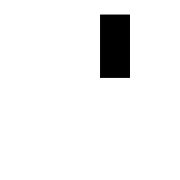
\includegraphics[width=\textwidth]{images/fingerprint_example.pdf}
\end{figure}
\begin{block}{Kernels used for the feature embedding in RankSVM}
\vspace{-0.25cm}
\begin{small}
\begin{itemize}
    \item Binary: Tanimoto kernel 
\begin{center}
    $\kmol(m_i,m_j)=\frac{b(m_i)^T b(m_j)}{b(m_i)^T b(m_i)+b(m_j)^T b(m_j)-b(m_i)^T b(m_j)}$
\end{center}
    \item Count: MinMax kernel 
\begin{center}
    $\kmol(m_i,m_j)=\frac{\sum_{s=1}^{N_{sub}}\min(c_s(m_i),c_s(m_j))}{\sum_{s=1}^{N_{sub}}\max(c_s(m_i),c_s(m_j))}$
\end{center}
\end{itemize}
\end{small}
\end{block}
}

\frame{ 
    \frametitle{Compare binary and counting molecular fingerprints}
%     \framesubtitle{Encoding molecular structures using MACCS dictionary molecular fingerprints.}

\begin{itemize}
    \item Pairwise prediction accuracy ($\pm 2\sigma$) for different target systems
    \item RankSVM models trained using single system $\Pref(\sys)$.
\end{itemize}

\begin{table}[!t]
\begin{tabular}{@{}lcc@{}}
    \toprule 
    Target system $\sys$ & Binary MACCS & Counting MACCS \\\midrule
    Eawag\_XBridgeC18 & $0.796 (\pm 0.015)$ & $\mathbf{0.844 (\pm 0.011)}$ \\
    FEM\_long         & $0.882 (\pm 0.016)$ & $\mathbf{0.905 (\pm 0.015)}$ \\
    RIKEN             & $0.826 (\pm 0.024)$ & $\mathbf{0.848 (\pm 0.017)}$ \\
    UFZ\_Phenomenex   & $0.790 (\pm 0.027)$ & $\mathbf{0.802 (\pm 0.017)}$ \\
    LIFE\_old         & $0.842 (\pm 0.050)$ & $\mathbf{0.862 (\pm 0.035)}$ \\
    \bottomrule
\end{tabular}
\end{table} 
}

\frame{
    \frametitle{Train model with preferences from different systems}
    \framesubtitle{Can pairwise predictor benefit from information of different systems?}

\begin{block}{Compare performance of different training sets}
\begin{itemize}
    \item Single system, target data only: $\Pref(\sys)$
    \item Multiple systems, \emph{no} target data: $\Pref\setminus\Pref(\sys)$
    \item Multiple systems, all available data: $\Pref$
    \item Varying percentage ???
\end{itemize}
\end{block}
\begin{block}{Comparison method}
\begin{itemize}
    \item Support Vector Regression (SVR) trained on retention times directly \cite{Aicheler2015}.
    \item In multiple system setting: Retention times are considered jointly.
\end{itemize}
\end{block}
}

\frame{
    \frametitle{Train model with preferences from different systems}
    \framesubtitle{Application setting: Training retention times only available from single target system.}
    
\begin{center}
    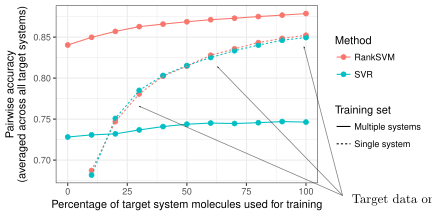
\includegraphics[width=\textwidth]{images/pwacc_2_marked_4.pdf}
\end{center}
\vspace{-0.25cm}
\begin{block}{Observations}
\begin{itemize}
    \item Increasing amount of training data improves prediction.
    \item RankSVM and SVR perform equally.
\end{itemize}
\end{block}
}

\frame{
    \frametitle{Train model with preferences from different systems}
    \framesubtitle{Application Setting: Training retention times only available \emph{from not target} system.}
    
\begin{center}
    \includegraphics[width=0.9\textwidth]{images/pwacc_2_marked_2.pdf}
\end{center}
\vspace{-0.25cm}
\begin{block}{Observations}
\begin{itemize}
    \item Performance of single system \emph{without} data from the target.
    \item RankSVM outperforms SVR by considering retention \emph{orders}.
\end{itemize}
\end{block}
}

\frame{
    \frametitle{Train model with preferences from different systems}
    \framesubtitle{Application Setting: Training retention times from target \emph{and} others systems available.}
    
\begin{center}
    \includegraphics[width=0.9\textwidth]{images/pwacc_2_marked_3.pdf}
\end{center}
\vspace{-0.25cm}
\begin{small}
\begin{block}{Observations}
\vspace{-0.15cm}
\begin{itemize}
    \item Considering target \emph{and} non-target systems' data outperforms single system.
    \item RankSVM again outperforms SVR.
\end{itemize}
\end{block}
\end{small}
}


\section[Data integration]{Integration of MS/MS scores \& retention orders}
% \frame{
%     \frametitle{\ex{``Classical'' MS/MS spectra based metabolite identification}}
%     
% \begin{figure}[t]
%     \centering
%     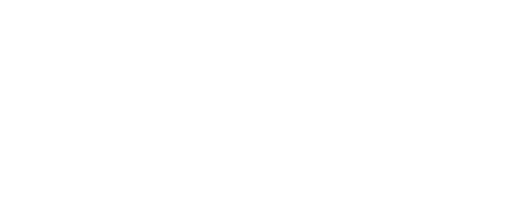
\includegraphics[width=1.0\textwidth]{images/molecular_candidates_only_iokr.pdf}
% \end{figure}    
% }
% 

\frame{
    \frametitle{Predicted retention orders for metabolite identification} 
%     \framesubtitle{Exploit observed retention order in complex LC-MS experiment}
    
\begin{figure}[t]
    \centering
    \includegraphics[width=0.8\textwidth]{images/lcms_spectrum_complex_small.pdf}
\end{figure}
\vspace{-0.15cm}
\begin{small}
\begin{block}{Identification workflow}
\vspace{-0.15cm}
\begin{enumerate}
    \item execute 1. (query candidates) and 2. (predict matching scores)
    \item Construct a layered graph:
\begin{itemize}
    \item Nodes: Molecular candidate structures $m_{i,j}$
    \item Edges: Encode matching scores and predicted retention orders   
\end{itemize}

    
%     where the nodes are molecular candidates and the edges encode the MS/MS matching scores as well as the predicted retention order.
%     \item Predict retention orders between all candidates $m_{i,j}$ and $m_{i+1,s}$ of MS/MS spectra of consecutively eluting molecules. \hfill\ex{$x_1$ and $x_2$}
    \item Find the \emph{overall} most consistent metabolite identification using the shorest path algorithm.
\end{enumerate}
\end{block}
\end{small}
}

\frame{
    \frametitle{\ex{Predicted retention orders for metabolite identification}} 
    
\only<1>{
\begin{figure}[c]
    \centering
    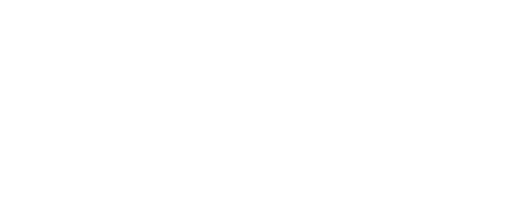
\includegraphics[width=0.9\textwidth]{images/molecular_candidates_no_shortest_path.pdf}
\end{figure}
}
\only<2>{
\begin{figure}[c]
    \centering
    \includegraphics[width=0.9\textwidth]{images/molecular_candidates.pdf}
\end{figure}
}
\vspace{-0.15cm}
\begin{small}
\begin{itemize}
    \item<1-> Edges connecting candidates of consecutive layers with edge weight:
\vspace{-0.25cm}
\begin{equation}
    \delta_{(i,j),(i+1,s)}=-y_{i+1,s}+D\cdot\max(0,\underbrace{\VEC{w}^T(\phi(m_{i,j})-\phi(m_{i+1,s})}_{\text{\alert<1>{RankSVM order penalty}}})),
\end{equation}
    $D\geq0$ weight on order penmalty: $\max(\ldots)>0$ if observed $\neq$ predicted order.
    \item<2> Candidates along the \alert<2>{shortest path} from first to last layer: \emph{most consistent identification}.
\end{itemize}
\end{small}

}

% \begin{block}{Retention order prediction function using RankSVM}
% \vspace{-0.5cm}
% \begin{equation}
%     f(\mol_i = \includegraphics[scale=1.2]{images/mol_i_unknown.pdf},\mol_j = \includegraphics[scale=1.2]{images/mol_j_unknown.pdf} ) 
%         = \begin{cases}
%             1  & \mol_i = \includegraphics[scale=1.2]{images/mol_i_unknown.pdf} \text{ elutes before } \mol_j = \includegraphics[scale=1.2]{images/mol_j_unknown.pdf}\\
%             -1 & \text{otherwise}
%         \end{cases}
% \end{equation}
% \end{block}


% Summary frame
\frame{
    \frametitle{Summary}
}

% Include references  
\printbibliography[heading=none]

\end{document}
